\documentclass[compress]{beamer}
\usepackage{ifthen,verbatim}

\title{Alignment update: CSA08 and CRUZET}
\author{Jim Pivarski, Alexei Safonov, K\'aroly Banicz$^*$}
\institute{Texas A\&M University, $^*$US-CMS}
\date{17 July, 2008}

\newcommand{\isnote}{}
\xdefinecolor{lightyellow}{rgb}{1.,1.,0.25}
\xdefinecolor{darkblue}{rgb}{0.1,0.1,0.7}

%% Uncomment this to get annotations
%% \def\notes{\addtocounter{page}{-1}
%%            \renewcommand{\isnote}{*}
%% 	   \beamertemplateshadingbackground{lightyellow}{white}
%%            \begin{frame}
%%            \frametitle{Notes for the previous page (page \insertpagenumber)}
%%            \itemize}
%% \def\endnotes{\enditemize
%% 	      \end{frame}
%%               \beamertemplateshadingbackground{white}{white}
%%               \renewcommand{\isnote}{}}

%% Uncomment this to not get annotations
\def\notes{\comment}
\def\endnotes{\endcomment}

\setbeamertemplate{navigation symbols}{}
\setbeamertemplate{headline}{\mbox{ } \hfill
\begin{minipage}{5.5 cm}
\vspace{-0.75 cm} \small
\end{minipage} \hfill
\begin{minipage}{4.5 cm}
\vspace{-0.75 cm} \small
\begin{flushright}
\ifthenelse{\equal{\insertpagenumber}{1}}{}{Jim Pivarski \hspace{0.2 cm} \insertpagenumber\isnote/\pageref{numpages}}
\end{flushright}
\end{minipage}\mbox{\hspace{0.2 cm}}\includegraphics[height=1 cm]{../cmslogo} \hspace{0.1 cm} \includegraphics[height=1 cm]{../tamulogo} \hspace{0.01 cm} \vspace{-1.05 cm}}

\begin{document}
\frame{\titlepage}

%% \begin{notes}
%% \item This is the annotated version of my talk.
%% \item If you want the version that I am presenting, download the one
%% labeled ``slides'' on Indico (or just ignore these yellow pages).
%% \item The annotated version is provided for extra detail and a written
%% record of comments that I intend to make orally.
%% \item Yellow notes refer to the content on the {\it previous} page.
%% \item All other slides are identical for the two versions.
%% \end{notes}

\begin{frame}
\frametitle{Main theme for this talk}
\small

Primary issue in alignment is not ``being too many radiation lengths
away from the reference system'' (multiple scattering), the issue is ``being
too close'' (dependence on fine details of the reference system)

\vspace{-0.15 cm}
\begin{center}
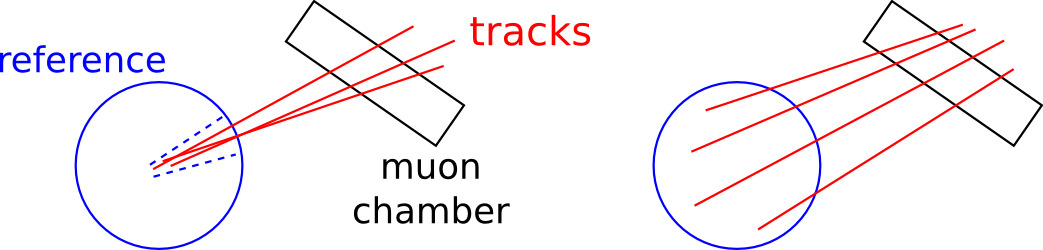
\includegraphics[width=0.7\linewidth]{limited_reference.png}
\end{center}

\vspace{-0.3 cm}
\begin{itemize}\setlength{\itemsep}{-0.075 cm}
\item Symmetric multiple scattering can be defeated with statistics
\item Dependence on reference can only be reduced by averaging over larger tracking volume
\end{itemize}

\vspace{0.1 cm}
\hspace{-0.83 cm} \textcolor{darkblue}{\Large Outline of topics}

\begin{itemize}\setlength{\itemsep}{-0.075 cm}
\item CSA08: results and lessons learned
\item CSC Overlaps procedure: what works, what doesn't, and why
\item Alignment with CRUZET data
\end{itemize}

\vspace{-1 cm}
\mbox{ }
\end{frame}

\begin{frame}
\frametitle{Last DPG presentation}
\small

Just before CSA08, things were changing quickly
\begin{itemize}
\item We found that the algorithm could be restored to a simpler state with improved resolution
\item Pre-CSA08 test yielded surprising results (multiple scattering had not been implemented in the 1\_8\_4 FastSim production)
\end{itemize}

\vspace{0.35 cm}
\hspace{-0.83 cm} \textcolor{darkblue}{\Large CSA08 exercise}

\begin{columns}
\column{0.4\linewidth}
\begin{itemize}
\item Included multiple scattering
\item First inclusive spectrum of muons (right)
\item First realistic tracker alignment $\to$ muon alignment workflow
\end{itemize}

\column{0.7\linewidth}
\mbox{ }

\vspace{0.35 cm}
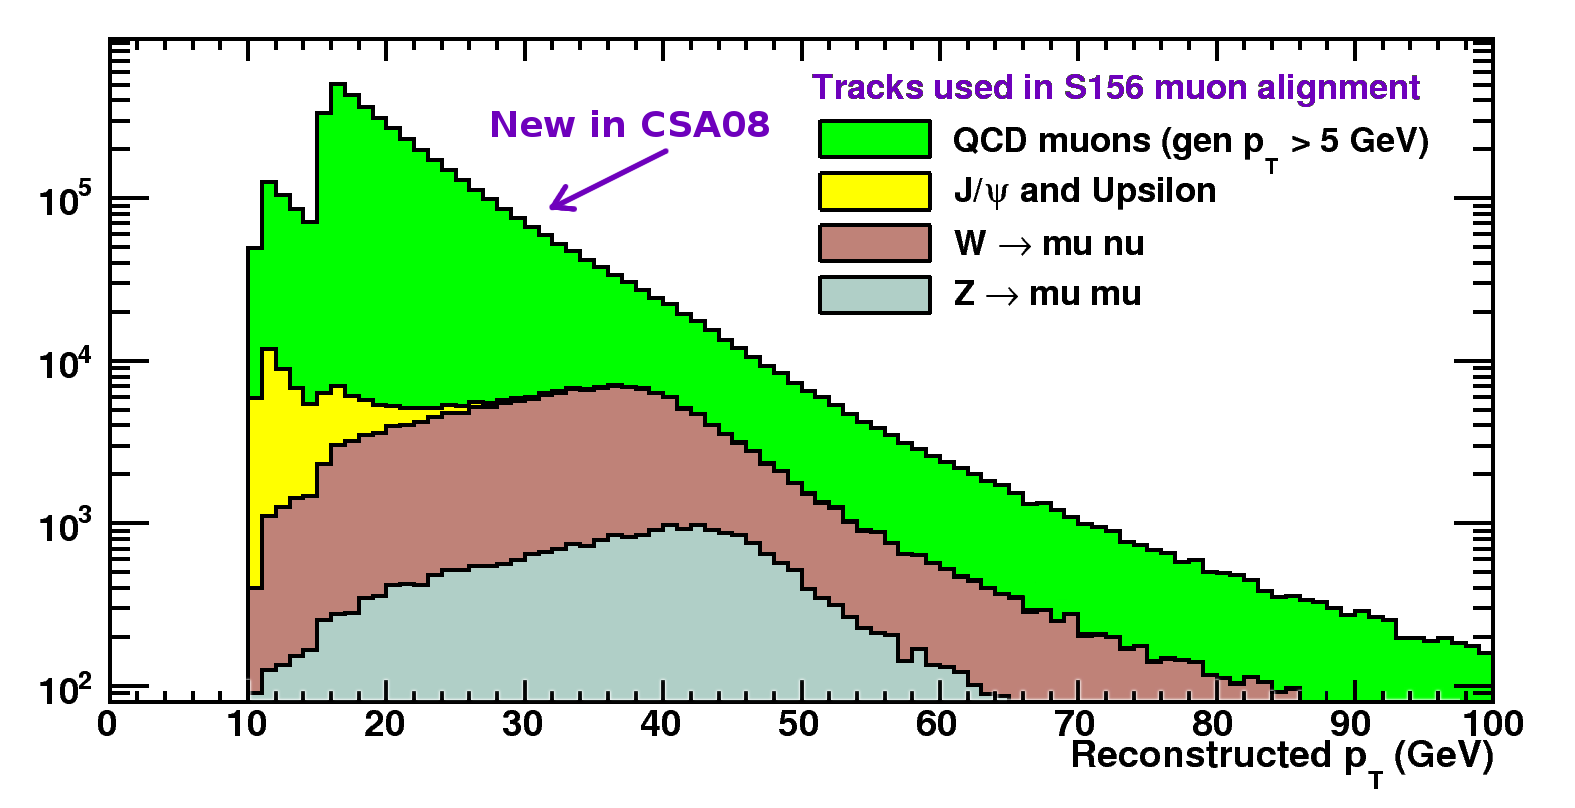
\includegraphics[width=\linewidth]{S156_pt_spectrum_noQCD5.png}
\end{columns}

\end{frame}

\begin{frame}
\frametitle{10~pb$^{-1}$ results}
\small
Histograms of aligned positions minus true positions in $r\phi$

MB1: 680~microns \hspace{0.3 cm} ME1/1: 520~microns \hspace{0.3 cm} ME1/2: 840~microns

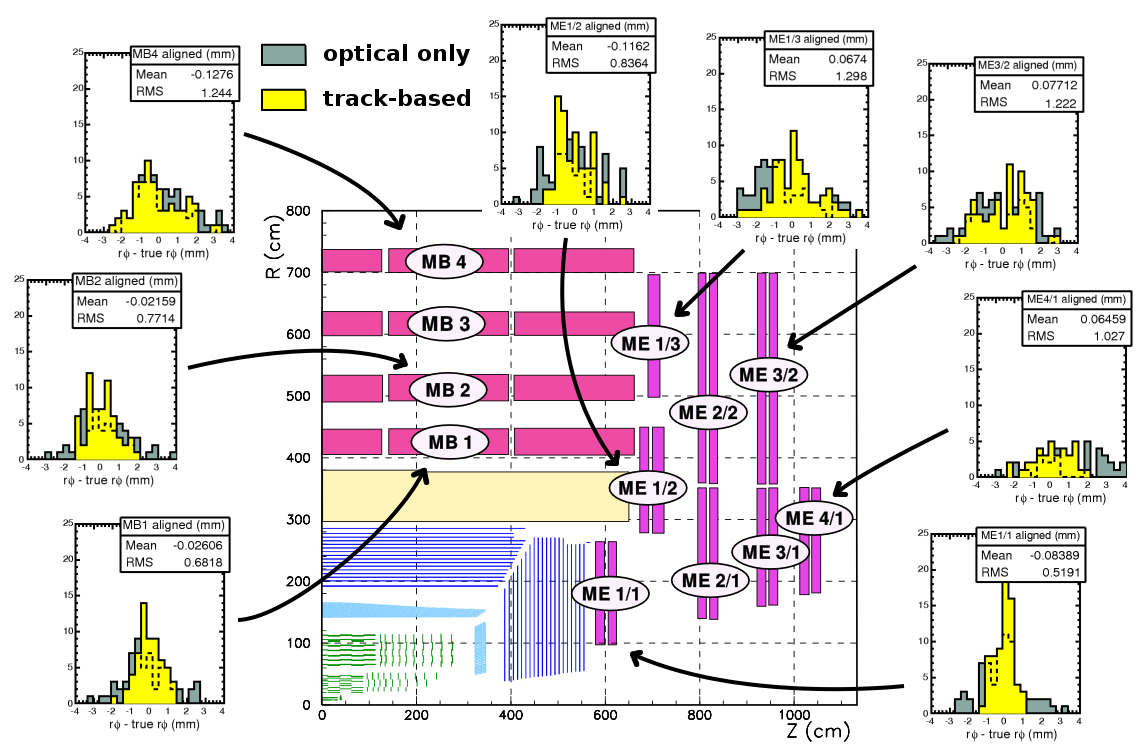
\includegraphics[width=\linewidth]{all_results_crop.png}
\end{frame}

\begin{frame}
\frametitle{Key result \#1}
\small

\textcolor{darkblue}{Long-standing question:} is it better\ldots
\begin{itemize}
\item to select high-momentum tracks and reduce multiple scattering (minimize standard deviation of residuals)
\item or open the floodgates and let in all muons (maximize $\sqrt{N}$)?
\end{itemize}

\vfill
Alignment correction is (roughly) mean of residual distribution,
\[ \mbox{uncertainty} = \frac{\mbox{standard deviation}}{\sqrt{N}} \]

\vfill
\textcolor{darkblue}{Answer:} open the floodgates (minimum $p_T$ of 10~GeV)

\vspace{0.1 cm}
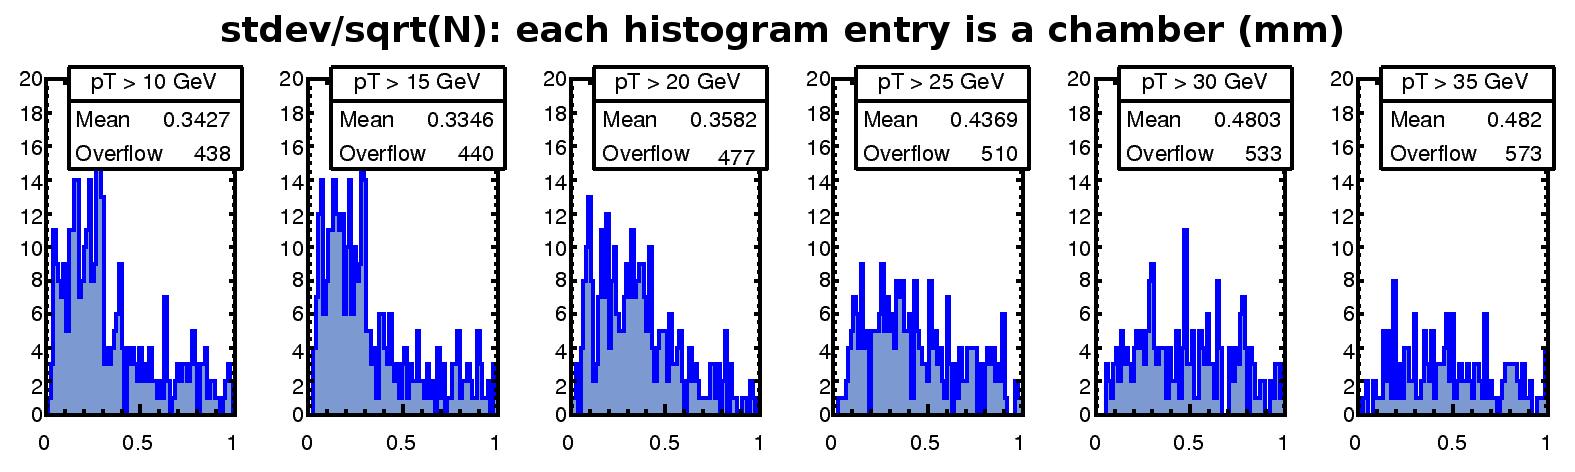
\includegraphics[width=\linewidth]{widening.png}
\end{frame}

\begin{frame}
\frametitle{Key result \#2}
\small

\hspace{-0.83 cm} \textcolor{darkblue}{\Large Strong dependence on tracker misalignment}

\vspace{0.25 cm} \renewcommand{\arraystretch}{0.6}
\begin{tabular}{p{0.45\linewidth} c p{0.45\linewidth}}
Previous studies used randomly-generated tracker misalignment scenarios & & models internal misalignment correlations expected from assembly \\

& & \\

New study uses output of tracker alignment algorithm as input to muon alignment & & includes correlations generated by tracker alignment attempt

\end{tabular}

\vspace{-0.1 cm}
\begin{center}
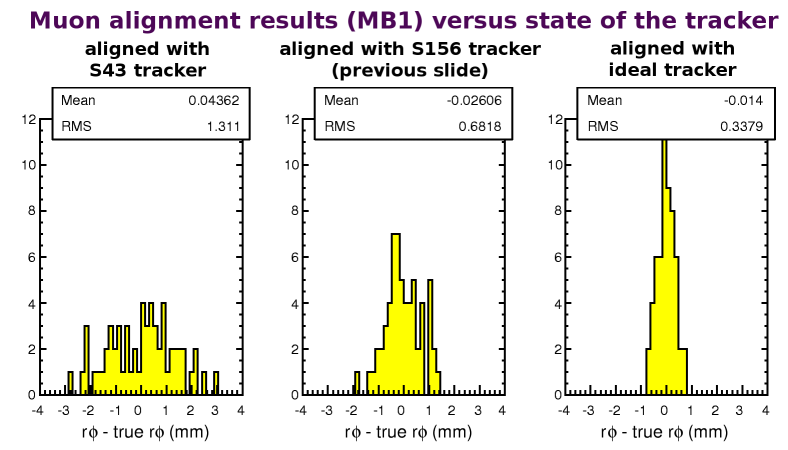
\includegraphics[width=0.7\linewidth]{muonalignment_MB1_dep_on_tracker.png}
\end{center}

\vspace{-1 cm}
\mbox{ }
\end{frame}

\begin{frame}
\frametitle{Analysis of \#2}
\small

\begin{itemize}
\item Alignment performed using tracks from the interaction point
\item Tracks that reach a given chamber all pass through the same slice of tracker (main theme)
\item Tracker misalignments are $\mathcal{O}(\mbox{10 $\mu$m})$, effect is 680~$\mu$m
\end{itemize}

Mismeasured $\phi$ or $\eta$: \hfill $\displaystyle 10\mbox{ $\mu$m}\, \left(\frac{\mbox{4 m inner muon station}}{\mbox{1 m tracker radius/half-length}}\right) = 14\mbox{ $\mu$m}$

\vspace{0.2 cm}
Mismeasured curvature: \hfill $\displaystyle 10\mbox{ $\mu$m}\, \left(\frac{\mbox{4 m inner muon station}}{\mbox{0.5 m tracker half-radius}}\right)^2 = 640\mbox{ $\mu$m}$

\begin{center}
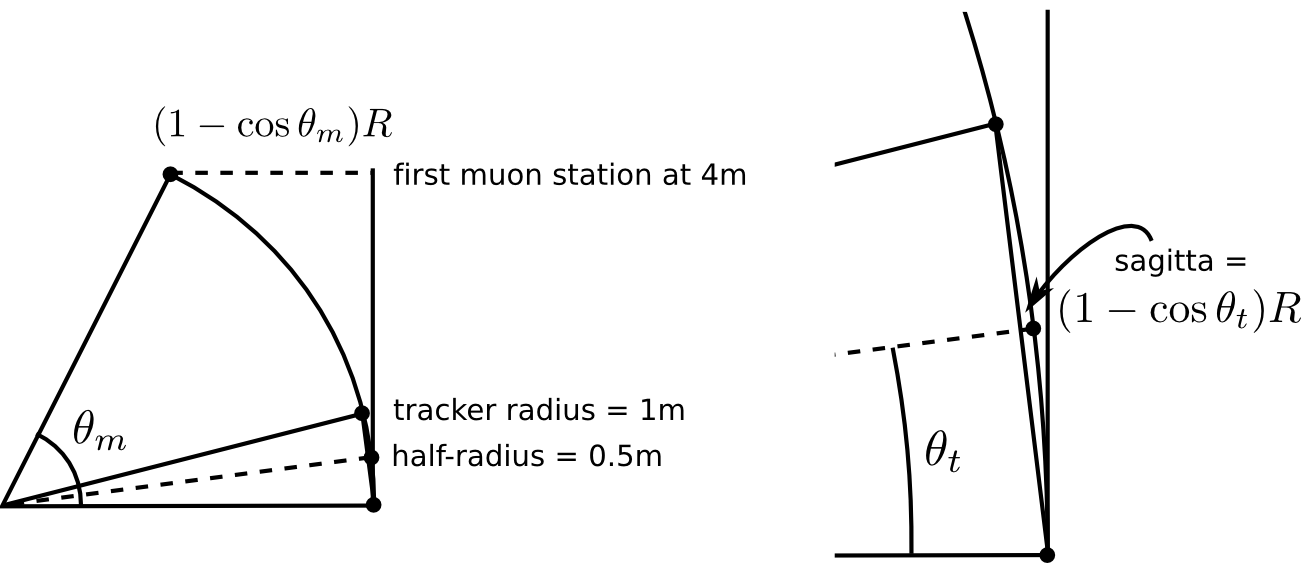
\includegraphics[width=0.7\linewidth]{curvature_extrapolation.png}
\end{center}
\end{frame}

\begin{frame}
\frametitle{What to do about it}
\small

\begin{enumerate}
\item Wait for tracker alignment to improve their curvature measurement (cosmic rays under-utilized in CSA exercise)
\item Improve tracker with muon system in combined fit \mbox{(tentatively discussed)\hspace{-1 cm}}
\item Average over tracker with $Z\to\mu\mu$ constraint

\begin{center}
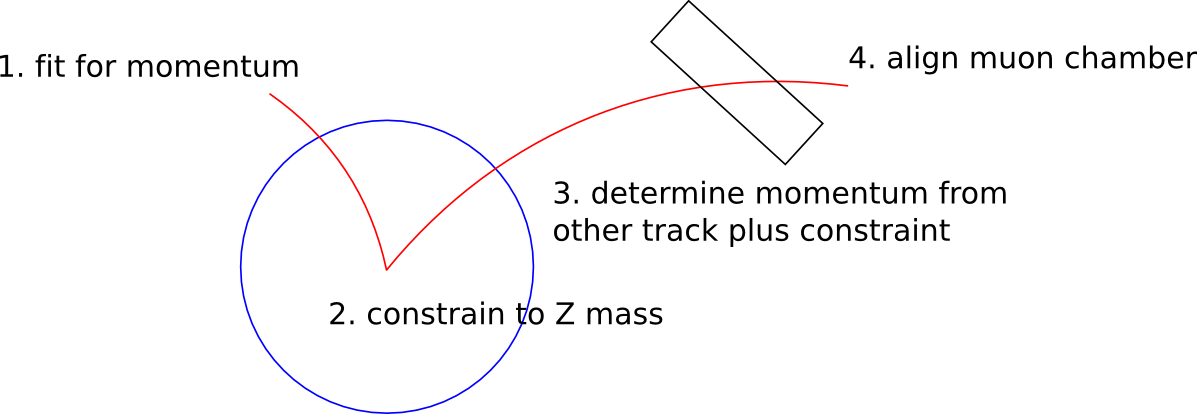
\includegraphics[height=2.3 cm]{Zmass_constraint.png}
\end{center}

\item Align with cosmic rays! (guaranteed high statistics, \mbox{best option for now)\hspace{-1 cm}}

\begin{center}
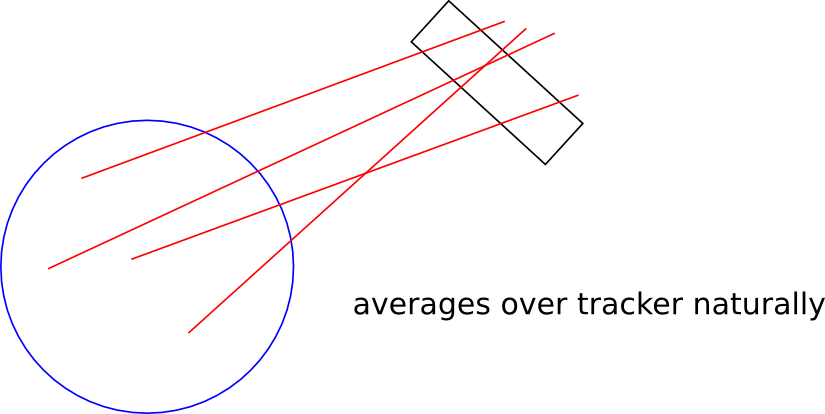
\includegraphics[height=2.3 cm]{cosmics_alignment.png}
\end{center}
\end{enumerate}

\end{frame}

\begin{frame}
\frametitle{CSC Overlaps procedure}
\small
\begin{columns}
\column{0.8\linewidth}
Basic idea: \hfill \textcolor{darkblue}{with Karoly Banicz}
\begin{itemize}
\item Relative alignment of pairs of CSCs using tracks that pass through the overlapping edges
\item Whole CSC rings can be aligned (internally) by propagating corrections around the ring
\end{itemize}

\column{0.2\linewidth}
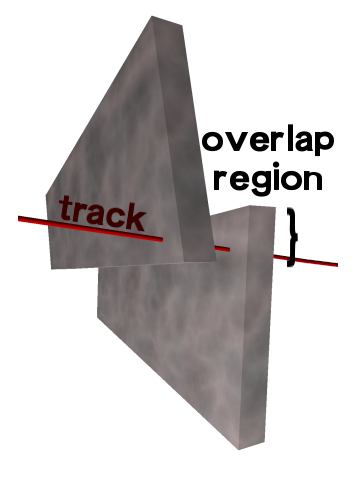
\includegraphics[width=\linewidth]{overlaps.png}
\end{columns}

\vfill
\hspace{-0.4 cm} History: (\textcolor{red}{$^*$} = discussed on subsequent slides)

\vspace{0.1 cm}
\renewcommand{\arraystretch}{1.2}
\begin{tabular}{l p{0.98\linewidth}}
& Old idea: chambers designed with overlap for this purpose \\
& This spring: beam-halo identified as a good source of tracks \\
& Many technical details, such as trigger \& AlCa paths to get these events \\
& Beam-halo MC AlCaReco descoped from CSA08 production, we reconstructed it ourselves \\
\textcolor{red}{$^*$} & Instability in ``even-odd'' procedure, replaced with ``one-sided'' procedure \\
\textcolor{red}{$^*$} & Specialized ``minitrack'' building in CRUZET data for efficiency \\
\textcolor{red}{$^*$} & CRUZET and MC converge, but rings do not close \\
\textcolor{red}{$^*$} & Granularity of wire groups might be responsible
\end{tabular}
\end{frame}

\begin{frame}
\frametitle{Even-odd procedure}

\begin{center}
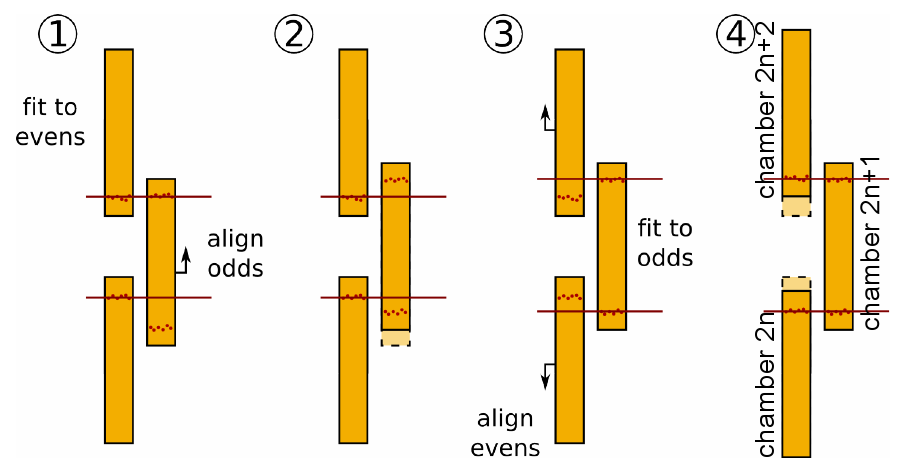
\includegraphics[width=0.6\linewidth]{even-odd.png}
\end{center}

\begin{columns}
\column{0.6\linewidth}
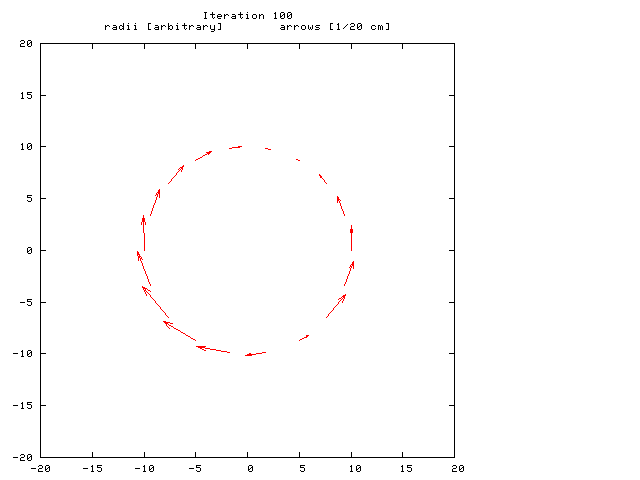
\includegraphics[width=\linewidth]{beamhalo_APE_r0_t100000_Xf0mm_iter100.png}

\column{0.4\linewidth}
\small
\begin{itemize}
\item Instability grows in ideal-geometry MC
\item This ``weak mode'' minimizes the mean by balancing left-edge residuals and right-edge residuals
\end{itemize}
\end{columns}
\end{frame}

\begin{frame}
\frametitle{One-sided procedure}

Don't mix left-edge residuals with right-edge residuals, and also align everything at once:

\vfill
\begin{center}
  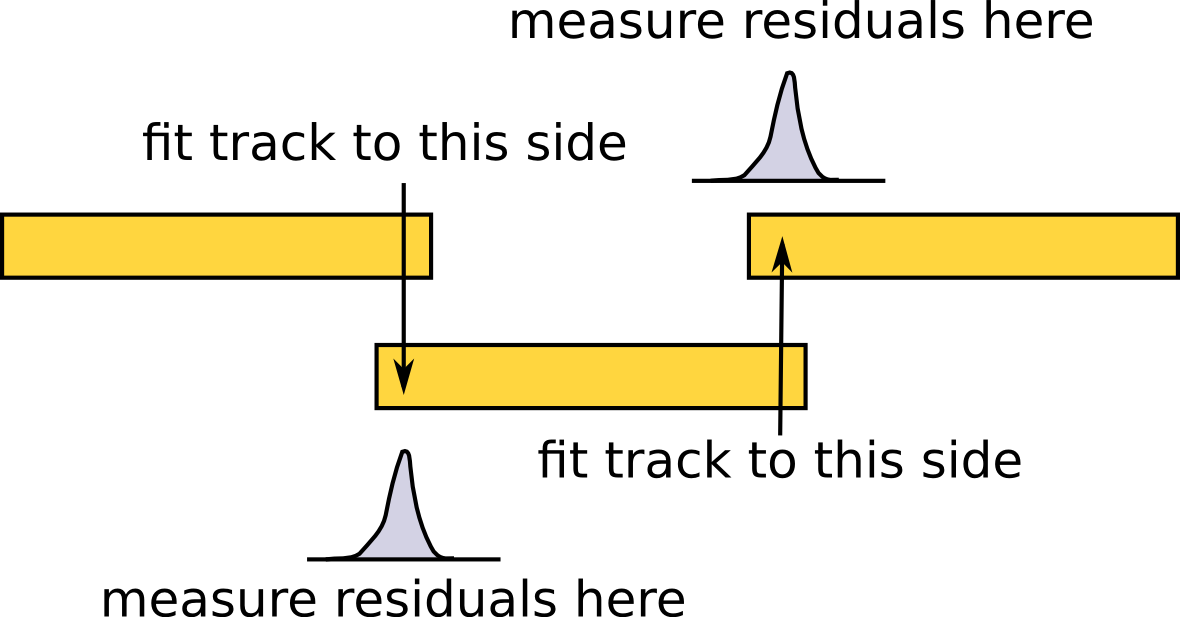
\includegraphics[width=0.6\linewidth]{fit_to_both.png}
\end{center}

\vfill
Reverse direction to quantify asymmetry

\vfill
This procedure converges in data and MC

(meaning: residuals are minimized and alignment stops)

\end{frame}

\begin{frame}
\frametitle{``Minitracks'' in CRUZET}
\small

\begin{itemize}
\item Overlap regions are narrow; cut has low acceptance
\item Full station-traversing muon tracks are not necessary, only need to match pairs of segments in overlapping chambers
\end{itemize}

Residuals on ME+4/1 chamber 16 from fit to chamber 15:
\begin{enumerate}
\item Any two segments in neighboring chambers
\item Exactly two segments, nearly collinear (linear fit has $\chi^2/\mbox{ndf}$ $<$ 10)
\item Aligned
\end{enumerate}

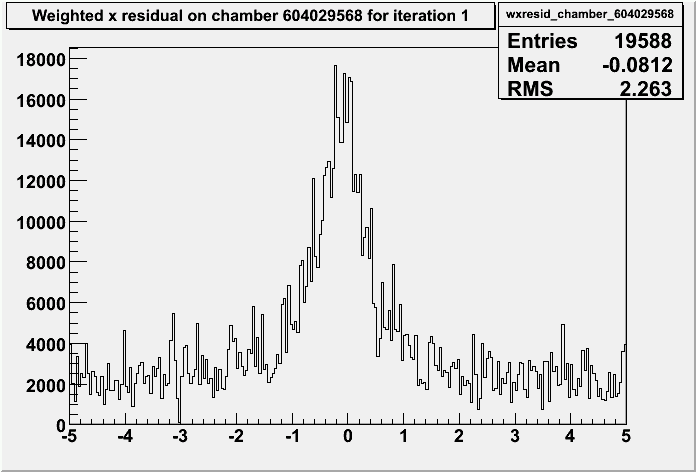
\includegraphics[height=3.5 cm]{before_cuts.png}
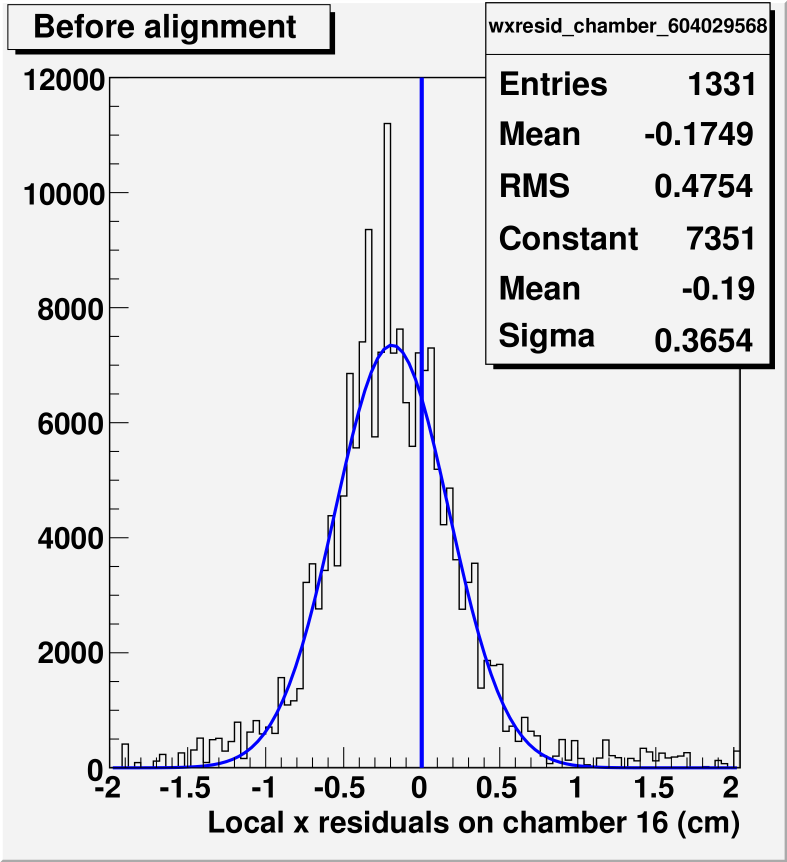
\includegraphics[height=3.5 cm]{before_alignment.png}
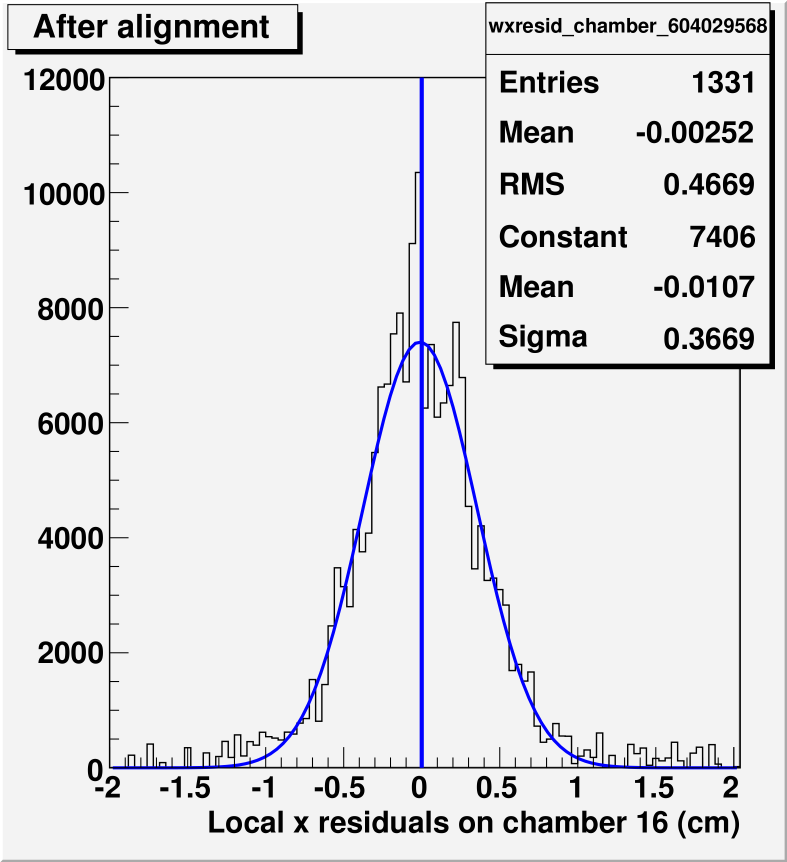
\includegraphics[height=3.5 cm]{after_alignment.png}

\end{frame}

\begin{frame}
\frametitle{Rings do not close}
\small

\begin{tabular}{p{0.5\linewidth} p{0.5\linewidth}}
ME+2/2 (CRUZET-1) & ME+3/2 (CRUZET-1) \\
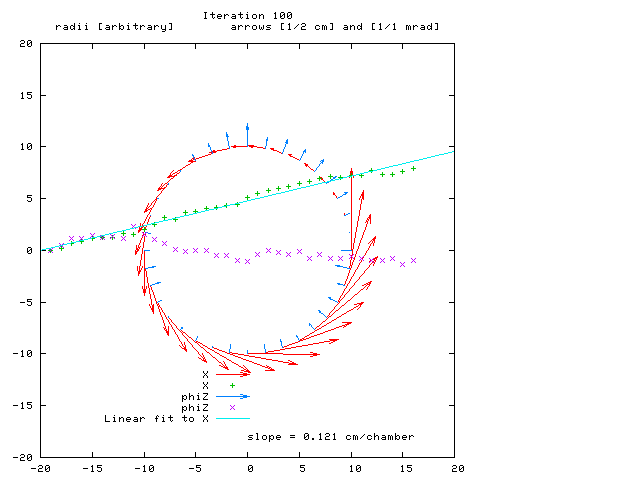
\includegraphics[width=\linewidth]{CRUZET1_MEplus22_plusIsRef_ch1fix_XphiZ.png} &
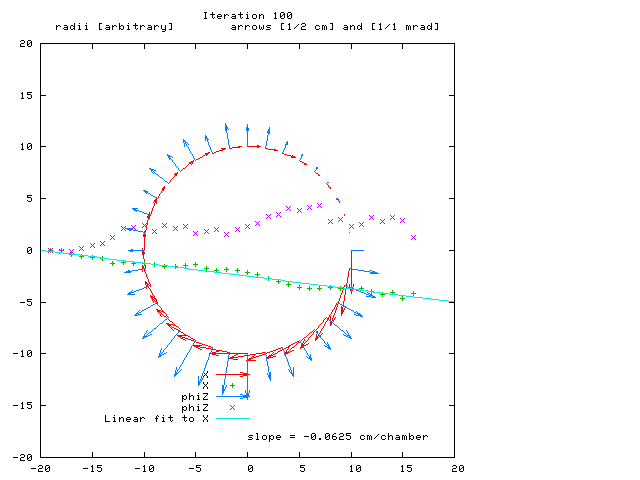
\includegraphics[width=\linewidth]{CRUZET1_MEplus32_plusIsRef_ch1fix_XphiZ.png}
\end{tabular}

\vspace{0.05 cm}
\begin{center}
Average alignment correction per chamber (confirmed in CRUZET-2)

\vspace{0.03 cm}
\renewcommand{\arraystretch}{1.2}
\begin{tabular}{c | c c c}
ring & ME+2 & ME+3 & ME+4 \\\hline
1 & $-0.5$~mm & ? & $+1.0$~mm \\
2 & $+1.2$~mm & $-0.6$~mm & \\
\end{tabular}
\end{center}

\vspace{0.05 cm} \scriptsize
{\it Iteration-by-iteration animations from CRUZET-1 and -2 available in}

\textcolor{blue}{\tt \underline{\href{https://banicz.web.cern.ch/banicz/CMS/alignment/CRUZET}{https://banicz.web.cern.ch/banicz/CMS/alignment/CRUZET}}}

\end{frame}

\begin{frame}
\frametitle{Interpretations}
\small

\begin{columns}
\column{0.5\linewidth}
ME+2/2 with $R += 6.6$~mm

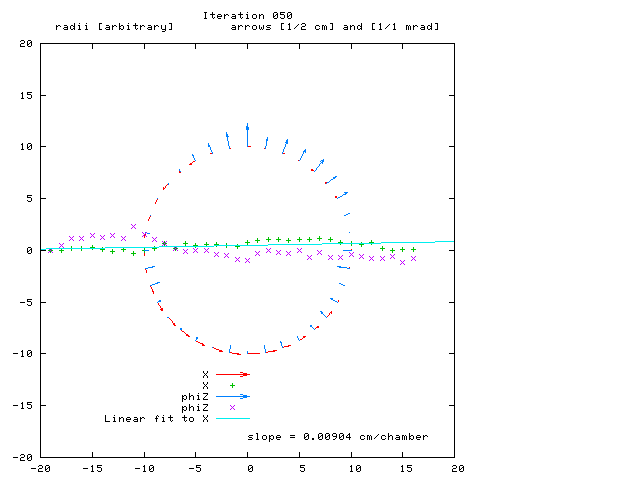
\includegraphics[width=\linewidth]{CRUZET1_MEplus22_Yf6_6mm_plusIsRef_ch1fix_XphiZ.png}

\column{0.5\linewidth}
Radial shift of all chambers in a ring?

\begin{center}
\renewcommand{\arraystretch}{1.2}
\begin{tabular}{c c}
ME+2/2 & ME+3/2 \\\hline
$+6.6$~mm & $-3$~mm
\end{tabular}
\end{center}

\begin{itemize}
\item How can these be in opposite directions?
\item Hard to imagine a transcription error or a physical effect which can do this
\end{itemize}
\end{columns}

\vfill
\begin{itemize}
\item Even less likely that all chambers are ``randomly'' misaligned by this same amount
\end{itemize}
\end{frame}

\begin{frame}
\frametitle{Wire group granularity?}

Perhaps the apparent radial shift is due to discrete wire groups

\begin{itemize}
\item for most hits, reconstructed $y$ is the nearest wire group center
\item at the edge of the chamber, $y$ is needed to resolve $x$
  position, propagating effect of granularity to $r\phi$
\end{itemize}

\vfill
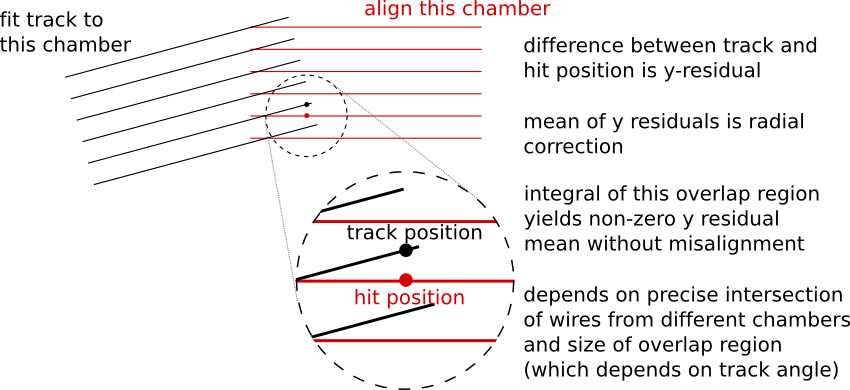
\includegraphics[width=\linewidth]{vertical_residual.png}

\end{frame}

\begin{frame}
\frametitle{Generating 6~mm shifts}
\small

\begin{itemize}
\item Beam-halo MC with ideal alignment
\item Overlay track extrapolated from reference (black) and hit (red)
\item Vertical difference between black and red is the $y$-residual
\item Can create a 6~mm $y$-residual by changing the degree of overlap
  (with cuts); cosmic rays have broader overlap due \mbox{to incidence angles\hspace{-1 cm}}
\end{itemize}

\mbox{ } \hfill 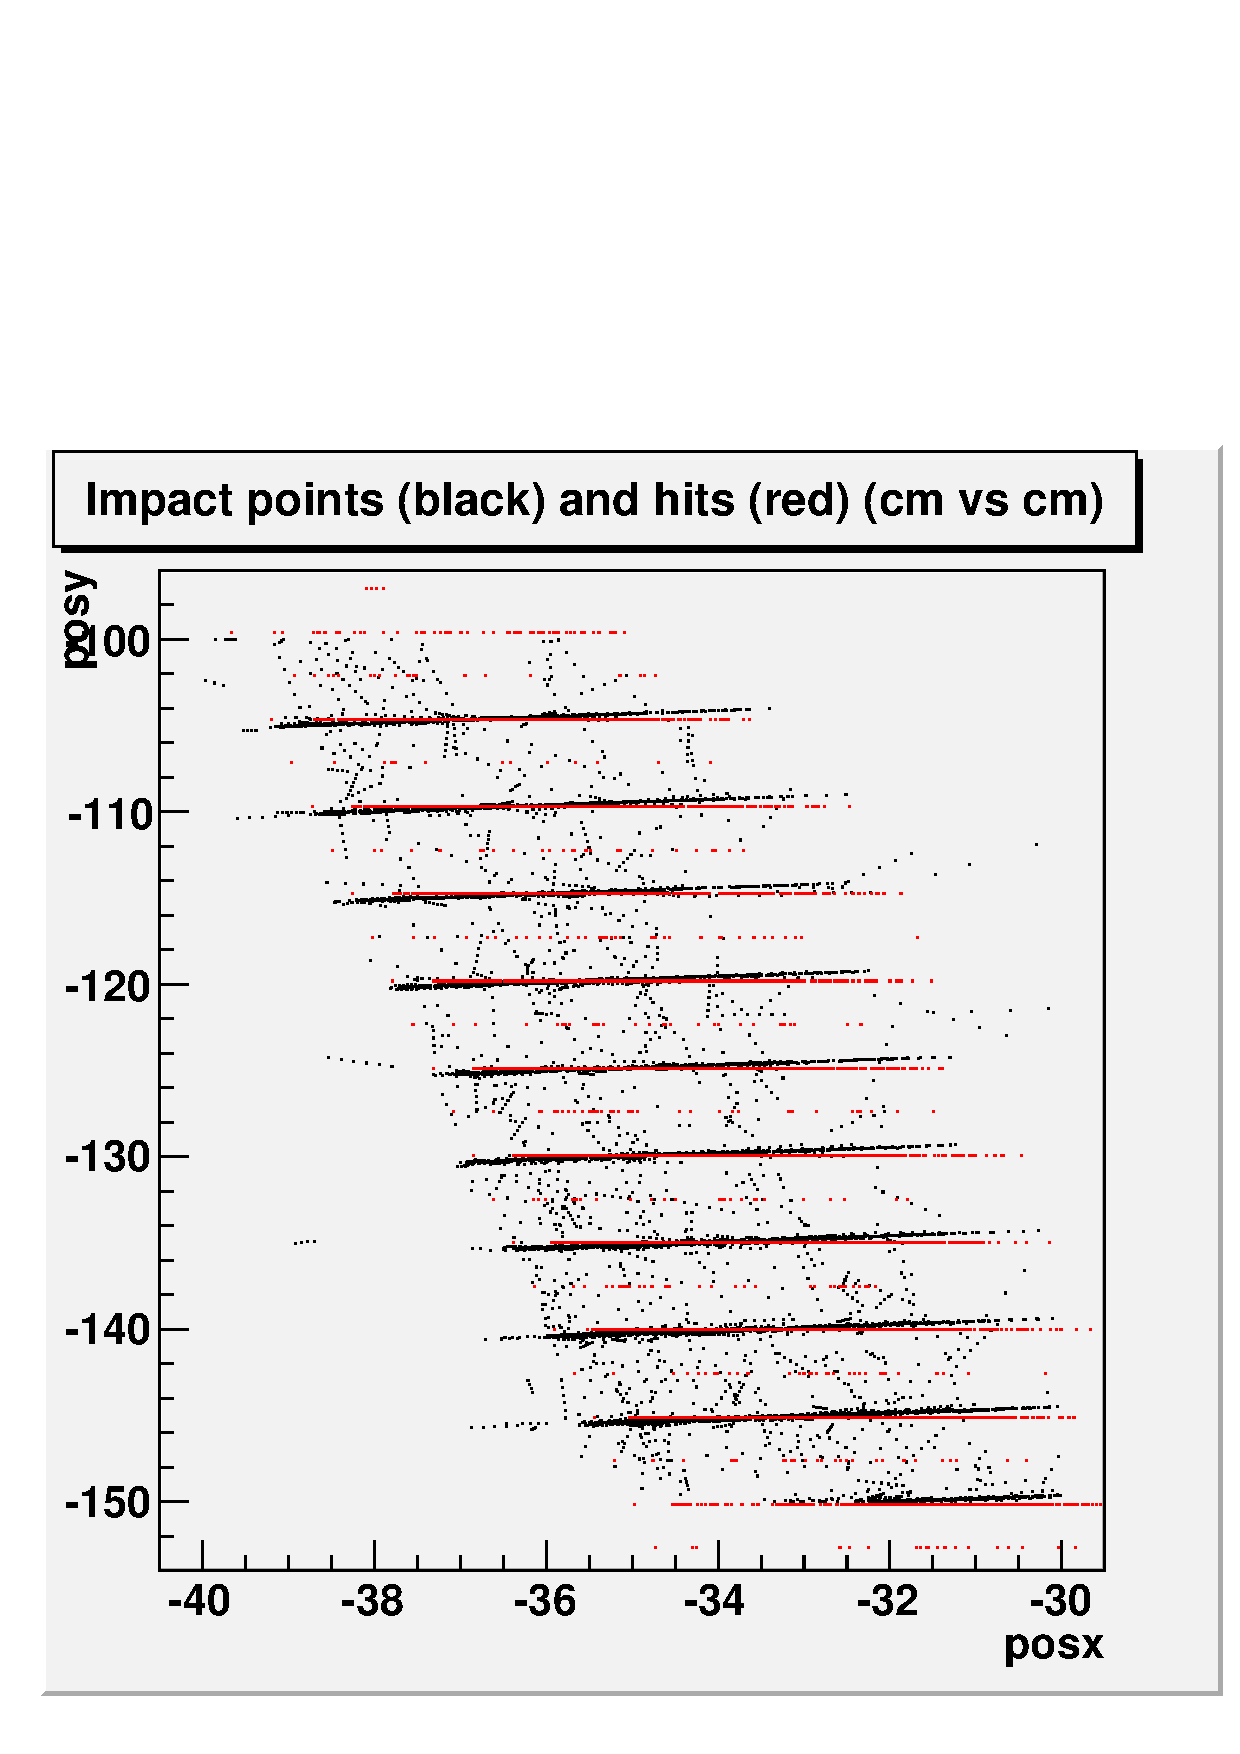
\includegraphics[width=0.45\linewidth]{selectioneffect_nocut.pdf}
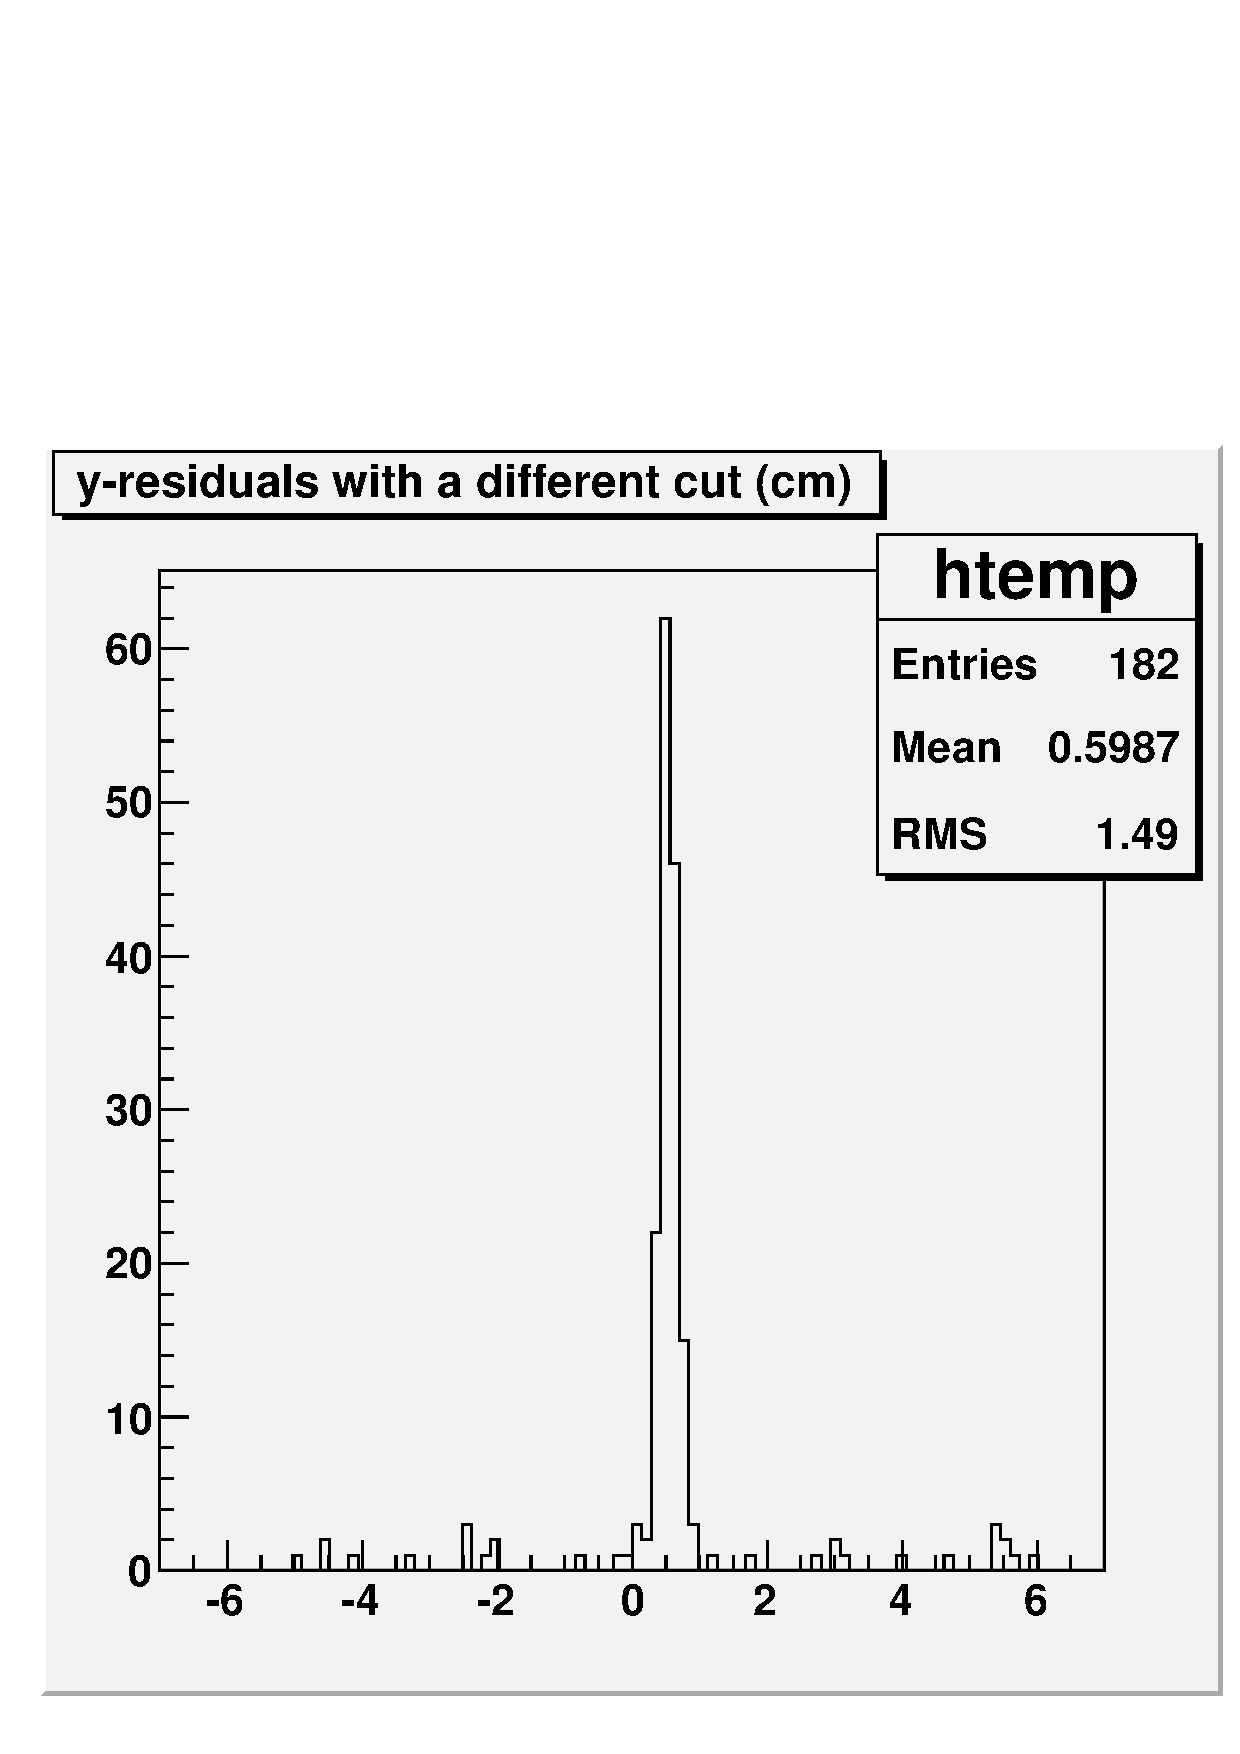
\includegraphics[width=0.45\linewidth]{selectioneffect_resid_withanothercut.pdf} \hfill \mbox{ }

\end{frame}

%% \section*{First section}
%% \begin{frame}
%% \begin{center}
%% \Huge \textcolor{blue}{First section}
%% \end{center}
%% \end{frame}

\begin{frame}
\frametitle{Next steps}
\small

\begin{itemize}
\item Apply baseline procedure to standAloneMuons in CRUZET-1/2 to look for the ``radial shift'' effect
\begin{itemize}
\item more affected by multiple scattering, but less affected by
  detailed structure of CSCs because we'll average over more chambers (main theme)
\end{itemize}

\vspace{-0.5 cm}
\begin{center}
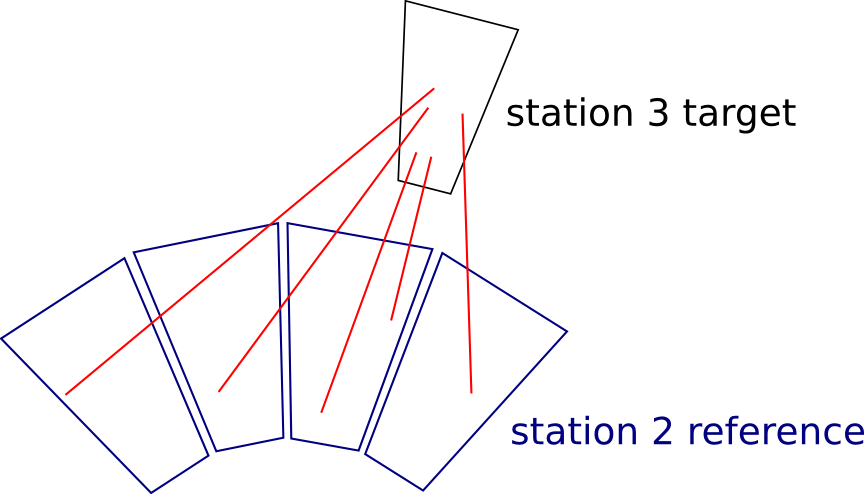
\includegraphics[width=0.5\linewidth]{baselineStandAloneMuons.png}
\end{center}

\item Ultimately, globalMuons from CRUZET-3 would have the least bias

\end{itemize}

\vspace{0.1 cm}
\hspace{-0.83 cm} \textcolor{darkblue}{\Large Conclusions}

\begin{itemize}
\item Settled final open MC questions in CSA08 exercise

\item Actively pursuing real-data alignments with CSC-overlaps procedure,
will test surprising outcome with the robust baseline procedure
\end{itemize}

\label{numpages}
\end{frame}

\end{document}
